% ---------------------------------------------------------------------
% Destaque colorido de um elemento de matriz: \destaque{cor}{conteúdo}
\providecommand{\destaque}[2]{{\setlength{\fboxsep}{1.5pt}\colorbox{#1}{$#2$}}}
\subsection{Ruído}\label{subsec:ruido-colorido}
% ---------------------------------------------------------------------
% ANTIGO:
% O equalizador LMMSE \textcolor{red}{(\textit{Linear Minimum Mean Square Error}) \cite{zhao2025jsac}} [] depende da matriz de covariância do ruído, que descreve suas características estatísticas e a relação entre os sinais observados nas diferentes antenas da \sout{estação base} \textcolor{red}{BS}. Quando o ruído é apenas térmico (AWGN) e por consequência, espacialmente branco, essa matriz é proporcional à identidade. Entretanto, a presença da interferência de usuários não-alvo adiciona correlação espacial do ruído entre as antenas. Esta seção apresenta o modelo de ruído considerado neste trabalho e deriva sua matriz de covariância.
\textcolor{red}{O equalizador LMMSE (\textit{Linear Minimum Mean Square Error}) depende da matriz de covariância do ruído \cite{zhao2025jsac}. Essa matriz descreve a potência do ruído em cada antena da BS e a relação entre as antenas. Quando o ruído é só térmico (AWGN), ela é proporcional à identidade. Os sinais dos UEs não-alvo também chegam às antenas da BS e tornam o ruído correlacionado entre elas. Neste trabalho, a soma dessa interferência com o ruído térmico é chamada de ruído colorido.}

\subsubsection{Ruído branco (AWGN)}
No modelo AWGN (Additive White Gaussian Noise), considera-se que o ruído é gaussiano, aditivo e espacialmente branco. Sua matriz de covariância é dada por:

\[
\mathbf R_n=\sigma^2\mathbf I_M,
\]

em que $\sigma^2$ representa a potência do ruído térmico por antena e $\mathbf I_M$ é a matriz identidade de dimensão $M\times M$. Como a matriz possui apenas elementos não nulos na diagonal, assume-se que os ruídos térmicos observados nas diferentes antenas são independentes. Nesse cenário, o equalizador LMMSE pode ser escrito como \cite{jeon2019}:

\[
\mathbf W_{\mathrm{LMMSE}}=
\left(
\mathbf H^H\mathbf H+
\rho\mathbf I_K
\right)^{-1}\mathbf H^H,
\]

em que  $\rho =  \dfrac{\sigma^2}{E_s}$, $E_s$ representa a energia média dos símbolos transmitidos e $K$ é o número de usuários alvo.

% ANTIGO:
% Entretanto, em cenários com interferência, o ruído térmico não é a única contribuição presente no sinal recebido. Os sinais transmitidos por usuários que não são alvos da detecção também chegam às antenas da \sout{estação base} \textcolor{red}{BS}. Como essas contribuições podem apresentar correção espacial, o ruído resultante deixa de ser branco. Neste trabalho, a combinação de interferência e ruído térmico é denominada ruído colorido.


\subsubsection{Assinatura espacial e Interferência}
% ANTIGO:
% O sinal transmitido por um \sout{equipamento de usuário} \textcolor{red}{UE} chega as M antenas da \sout{estação base} \textcolor{red}{BS}, multiplicado em cada antena pelo ganho do canal de propagação. Para um únco transmissor, o sinal recebido é:
\textcolor{red}{O sinal de um UE chega às $M$ antenas da BS multiplicado pelo ganho do canal em cada antena. Para um único transmissor, o sinal recebido é:}

\[
\mathbf y=\mathbf h s+\mathbf n,
\]

% ANTIGO:
% em que em que $\mathbf h\in\mathbb C^{M\times1}$ reúne os ganhos do canal entre o transmissor e as antenas da \sout{estação base} \textcolor{red}{BS}. Esse vetor é denomidado assinatura espacial do sinal, porque descreve como o sinal de um usuário se distribui pelo conjunto de antenas.
\textcolor{red}{em que $\mathbf h\in\mathbb C^{M\times1}$ reúne esses ganhos. Esse vetor é denominado assinatura espacial, porque descreve como o sinal do UE se distribui pelas antenas.}

% ANTIGO:
% Os UEs não-alvo da \sout{estação base} \textcolor{red}{BS} também tem a sua assinatura espacial e o sinal de cada $r$ usuário interferente chega a todas as antenas, com ganhos distintos entre elas. Assim, a mesma interferência ocorre simultaneamente em todas as antenas, o que a torna correlacionada entre elas. O ruído térmico, por outro lado, é gerado de forma independente em cada antena.
\textcolor{red}{Cada um dos $r$ UEs não-alvo também tem sua assinatura espacial. Assim, a mesma interferência chega a todas as antenas, com ganhos diferentes, e fica correlacionada entre elas. Já o ruído térmico é independente em cada antena.}

Pode-se definir o modelo de sinal recebido no cenário de interferência como:

\[
\mathbf y=
\mathbf H\mathbf s+\mathbf n=
\mathbf H\mathbf s+
\overline{\mathbf H}\,\overline{\mathbf s}
+\overline{\mathbf n},
\]

em que $\mathbf H\in\mathbb C^{M\times K}$ é a matriz de canal dos $K$ usuários-alvo, $\mathbf s\in\mathbb C^{K\times1}$ é o vetor de símbolos transmitidos por esses usuários, $\overline{\mathbf H}\in\mathbb C^{M\times r}$ representa os canais dos usuários interferentes e $\overline{\mathbf s}\in\mathbb C^{r\times1}$ reúne seus símbolos transmitidos. O vetor $\overline{\mathbf n}\in\mathbb C^{M\times1}$ representa o ruído térmico nas antenas receptoras.

\[
\overline{\mathbf H}=
\underbrace{\begin{bmatrix}
\bar h_{11} & \cdots & \bar h_{1r}\\
\vdots & \ddots & \vdots\\
\bar h_{M1} & \cdots & \bar h_{Mr}
\end{bmatrix}}_{M\times r},
\qquad
\overline{\mathbf s}=
\underbrace{\begin{bmatrix}\bar s_1\\ \vdots\\ \bar s_r\end{bmatrix}}_{r\times 1},
\qquad
\overline{\mathbf n}=
\underbrace{\begin{bmatrix}\bar n_1\\ \vdots\\ \bar n_M\end{bmatrix}}_{M\times 1}.
\]

Para construir o modelo do ruído colorido, considera-se que os usuários interferentes transmitem de forma independente com potência média $\beta$, de modo que:

\[
\mathbb E[\overline{\mathbf s}\,\overline{\mathbf s}^{H}]
=\beta\mathbf I_r=
\underbrace{\begin{bmatrix}
\destaque{orange!40}{\beta} & \cdots & 0\\
\vdots & \ddots & \vdots\\
0 & \cdots & \destaque{orange!40}{\beta}
\end{bmatrix}}_{r\times r}.
\]

Os elementos em destaque na diagonal são a potência $\beta$ de cada interferente. Os zeros fora da diagonal indicam que os interferentes são independentes entre si.


% ANTIGO:
% Assume-se também que o ruído térmico é espacialmente branco, com média nula e matriz de covariância:
%
% \[
% \mathbb E[\overline{\mathbf n}\,\overline{\mathbf n}^{H}]
% =\sigma^2\mathbf I_M=
% \underbrace{\begin{bmatrix}
% \destaque{yellow!40}{\sigma^2} & \cdots & 0\\
% \vdots & \ddots & \vdots\\
% 0 & \cdots & \destaque{yellow!40}{\sigma^2}
% \end{bmatrix}}_{M\times M}.
% \]
%
% Os elementos em destaque na diagonal são a potência $\sigma^2$ do ruído térmico em cada antena. Os zeros fora da diagonal indicam que o ruído de uma antena não depende do ruído das outras.
%
% Além disso, os símbolos dos interferentes e o ruído térmico são considerados mutuamente independentes e de média nula. A matriz de canal $\overline{\mathbf H}$ é tratada como constante durante o intervalo de coerência considerado.
\textcolor{red}{O ruído térmico tem média nula e covariância $\sigma^2\mathbf I_M$, como no modelo AWGN. Os símbolos dos interferentes e o ruído térmico são independentes entre si e de média nula. A matriz $\overline{\mathbf H}$ é constante durante o intervalo de coerência.}


\subsubsection{Matriz de covariância do ruído}
% ANTIGO:
% O ruído colorido é definido pela soma das contribuições dos usuários interferentes e do ruído térmico:
%
% \[
% \mathbf n=
% \overline{\mathbf H}\,\overline{\mathbf s}
% +\overline{\mathbf n}.
% \]
%
% Sua matriz de covariância é dada por:
%
% \[
% \mathbf R_n
% \triangleq
% \mathbb E[\mathbf n\mathbf n^H].
% \]
%
% Como as duas parcelas são independentes e possuem média nula, a covariância da soma é igual à soma de suas covariâncias. Portanto,
\textcolor{red}{O ruído colorido é $\mathbf n=\overline{\mathbf H}\,\overline{\mathbf s}+\overline{\mathbf n}$, e sua matriz de covariância é $\mathbf R_n\triangleq\mathbb E[\mathbf n\mathbf n^H]$. Como as duas parcelas são independentes e de média nula, a covariância da soma é a soma das covariâncias:}

\[
\mathbf R_n=
\operatorname{Cov}
\left(\overline{\mathbf H}\,\overline{\mathbf s}\right)
+
\operatorname{Cov}(\overline{\mathbf n}).
\]

A primeira parcela pode ser obtida pela propriedade da covariância sob uma transformação linear. Para uma matriz determinística $\mathbf A$ e um vetor aleatório $\mathbf z$, vale:

\[
\operatorname{Cov}(\mathbf A\mathbf z)=
\mathbf A\operatorname{Cov}(\mathbf z)\mathbf A^H.
\]

Aplicando essa propriedade à contribuição dos interferentes, obtém-se:

\[
\begin{aligned}
\operatorname{Cov}
\left(\overline{\mathbf H}\,\overline{\mathbf s}\right)
&=
\overline{\mathbf H}
\mathbb E[\overline{\mathbf s}\,\overline{\mathbf s}^H]
\overline{\mathbf H}^H\\
&=
\beta\overline{\mathbf H}\,\overline{\mathbf H}^H.
\end{aligned}
\]

Como a covariância do ruído térmico é $\sigma^2\mathbf I_M$, a matriz de covariância do ruído colorido resulta em:

\[
\boxed{
\mathbf R_n=
\beta\overline{\mathbf H}\,\overline{\mathbf H}^H
+\sigma^2\mathbf I_M
}
\]

\[
\underbrace{\overline{\mathbf H}}_{M\times r}\,
\underbrace{\beta\mathbf I_r}_{r\times r}\,
\underbrace{\overline{\mathbf H}^H}_{r\times M}
+
\underbrace{\sigma^2\mathbf I_M}_{M\times M}
=
\underbrace{\begin{bmatrix}
r_{11} & \destaque{green!30}{r_{12}} & \cdots & \destaque{green!30}{r_{1M}}\\
\destaque{green!30}{r_{21}} & r_{22} & \cdots & \destaque{green!30}{r_{2M}}\\
\vdots & \vdots & \ddots & \vdots\\
\destaque{green!30}{r_{M1}} & \destaque{green!30}{r_{M2}} & \cdots & r_{MM}
\end{bmatrix}}_{\mathbf R_n\ (M\times M)}
\]

% ANTIGO:
% A matriz $\mathbf R_n$ possui dimensão $M\times M$ e reúne duas contribuições distintas. O termo $\sigma^2\mathbf I_M$ representa o ruído térmico, cuja covariância é nula entre antenas distintas. Já o termo $\beta\overline{\mathbf H}\,\overline{\mathbf H}^H$ representa a covariância da interferência recebida. Como cada sinal interferente pode ser observado simultaneamente por várias antenas, essa parcela pode apresentar elementos não nulos fora da diagonal, indicando correlação espacial. Na matriz acima, esses são os elementos em destaque: cada um indica o quanto o ruído de duas antenas distintas está correlacionado. Os elementos da diagonal, sem destaque, são a potência do ruído em cada antena.
%
% Assim, a matriz $\mathbf R_n$ descreve tanto a potência do ruído em cada antena quanto as relações estatísticas entre as diferentes componentes do vetor de ruído. Essa informação é necessária para modelar adequadamente a interferência no equalizador LMMSE. Sob a hipótese de símbolos-alvo independentes, com covariância $E_s\mathbf I_K$ e independentes do ruído, a matriz de covariância do sinal recebido fica:
%
% \[
% \mathbf R_y=
% E_s\mathbf H\mathbf H^H+\mathbf R_n,
% \]
%
% ou, equivalentemente,
%
% \[
% \mathbf R_y=
% E_s\mathbf H\mathbf H^H+
% \beta\overline{\mathbf H}\,\overline{\mathbf H}^H
% +\sigma^2\mathbf I_M.
% \]
\textcolor{red}{O termo $\sigma^2\mathbf I_M$ só contribui para a diagonal. Já o termo $\beta\overline{\mathbf H}\,\overline{\mathbf H}^H$, da interferência, pode ter elementos não nulos fora da diagonal. Na matriz acima, esses são os elementos em destaque: cada um indica o quanto o ruído de duas antenas está correlacionado. Os elementos da diagonal são a potência do ruído em cada antena.}

\textcolor{red}{O equalizador LMMSE usa essa matriz para levar a interferência em conta. Se os símbolos-alvo são independentes, com covariância $E_s\mathbf I_K$, e independentes do ruído, a matriz de covariância do sinal recebido é:}

\[
\mathbf R_y=
E_s\mathbf H\mathbf H^H+\mathbf R_n=
E_s\mathbf H\mathbf H^H+
\beta\overline{\mathbf H}\,\overline{\mathbf H}^H
+\sigma^2\mathbf I_M.
\]



\subsubsection{Interferência sobre ruído térmico (\texorpdfstring{\textcolor{red}{IoTh}}{IoTh})}
A \textcolor{red}{IoTh} mede a intensidade da interferência em relação ao ruído térmico. Ela é definida como \cite{zhao2025jsac}:

\begin{equation}
\textcolor{red}{\mathrm{IoTh}}=10\log_{10}\left(\frac{\beta+N_0}{\sigma^2}\right),\label{eq:iot}
\end{equation}

em que $N_0$ é a potência do ruído térmico, ou seja, $N_0=\sigma^2$, assim como na SNR medida por $E_s/N_0$ em \cite{zhao2021-globecom}.

A potência $\beta$ dos UEs não-alvo controla a intensidade da interferência. Quando a \textcolor{red}{IoTh} é baixa, $\mathbf R_n$ se aproxima de $\sigma^2\mathbf I_M$ e o ruído é praticamente branco. À medida que a \textcolor{red}{IoTh} cresce, a parcela $\beta\overline{\mathbf H}\,\overline{\mathbf H}^H$ domina e a correlação entre as antenas se torna mais forte.

\subsubsection{Estimação da matriz de covariância}\label{subsubsec:estimacao-R}
% aqui eh o lugar para explicar RCC
% explicar tambem a quantidade de pilotos e etc
% ANTIGO:
% A matriz $\mathbf R_n$ é uma grandeza teórica, definida por uma esperança, o que exigiria infinitas realizações do ruído, além de depender dos canais $\overline{\mathbf H}$ dos usuários interferentes e de sua potência de transmissão $\beta$ que o receptor não conhece. Por isso, $\mathbf R_n$ precisa ser estimada a partir de observações de amostras do ruído observadas pelo receptor.
\textcolor{red}{A matriz $\mathbf R_n$ é definida por uma esperança e depende de $\overline{\mathbf H}$ e de $\beta$, que o receptor não conhece. Por isso, o receptor estima $\mathbf R_n$ a partir de amostras do ruído.}

A estimativa amostral é dada por:

\[
\widehat{\mathbf R}_n=
\frac{1}{N}
\sum_{i=1}^{N}
\mathbf n^i(\mathbf n^i)^H,
\]

% ANTIGO:
% em que $N$ é o número de amostras disponíveis e $\mathbf n^i\in\mathbb C^{M\times1}$ representa a $i$-ésima amostra de ruído colorido. Cada amostra corresponde a uma observação do ruído nas $M$ antenas da \sout{estação base} \textcolor{red}{BS}.
\textcolor{red}{em que $N$ é o número de amostras e $\mathbf n^i\in\mathbb C^{M\times1}$ é a $i$-ésima amostra de ruído colorido, observada nas $M$ antenas da BS.}


% ANTIGO:
% As amostras de ruído são obtidas durante a transmissão de símbolos piloto. Como o sinal transmitido pelos usuários-alvo é conhecido pelo receptor nessa etapa, sua contribuíção pode ser removida do sinal recebido. O resíduo contém a interferência dos usuários não-alvo somada ao ruído térmico, constituindo a amostra de ruído colorido utilizada na estimação.
\textcolor{red}{As amostras vêm dos símbolos piloto. Nesses símbolos, o receptor conhece o sinal dos UEs alvo e pode removê-lo do sinal recebido. O que sobra é a interferência mais o ruído térmico, ou seja, uma amostra de ruído colorido.}

O produto externo de uma amostra por sua transposta conjugada, $\mathbf n^i(\mathbf n^i)^H$, produz uma matriz de dimensão $M\times M$. Cada elemento dessa matriz corresponde ao produto entre o ruído observado em duas antenas na mesma amostra:

\[
\left[\mathbf n^i(\mathbf n^i)^H\right]_{ab}=
n_a^i(n_b^i)^*.
\]

\[
\underbrace{\begin{bmatrix} n_1^i\\ n_2^i\\ \vdots\\ n_M^i\end{bmatrix}}_{M\times 1}
\underbrace{\begin{bmatrix} (n_1^i)^* & (n_2^i)^* & \cdots & (n_M^i)^*\end{bmatrix}}_{1\times M}
=
\underbrace{\begin{bmatrix}
\destaque{yellow!40}{n_1^i(n_1^i)^*} & n_1^i(n_2^i)^* & \cdots & n_1^i(n_M^i)^*\\
n_2^i(n_1^i)^* & \destaque{yellow!40}{n_2^i(n_2^i)^*} & \cdots & n_2^i(n_M^i)^*\\
\vdots & \vdots & \ddots & \vdots\\
n_M^i(n_1^i)^* & n_M^i(n_2^i)^* & \cdots & \destaque{yellow!40}{n_M^i(n_M^i)^*}
\end{bmatrix}}_{M\times M}
\]

Quando $a=b$, o produto corresponde à potência observada na antena considerada. Esses são os elementos em destaque na diagonal da matriz acima. Quando $a\neq b$, o produto relaciona os sinais de ruído observados em duas antenas distintas.

% ANTIGO:
% A média desses produtos ao longo das $N$ amostras fornece uma estimativa dos elementos correspondentes de $\mathbf R_n$. Dessa forma, cada amostra contribui para a estimação da potência do ruído em cada antena e das relações estatísticas entre pares de antenas. Uma única observação não é suficiente para caracterizar essas propriedades estatísticas; a estimativa torna-se mais representativa à medida que são incorporadas novas amostras. Ou seja, a qualidade da estimativa depende do número de amostras utilizadas.
%
% A quantidade de amostras, no entanto, é limitada pelos recursos disponíveis para a coleta. No sistema considerado, as amostras são obtidas a partir de elementos de recurso de pilotos, cuja disponibilidade depende da configuração do sinal e do intervalo durante o qual a covariância pode ser considerada constante.
\textcolor{red}{A média desses produtos ao longo das $N$ amostras estima cada elemento de $\mathbf R_n$. Uma única amostra não basta, e a estimativa melhora à medida que $N$ cresce.}


\subsubsection{Availability of noise samples within the coherence time}\label{subsubsec:disponibilidade-amostras}
All samples used in noise estimation must represent the same covariance matrix. Therefore, the sampling interval is limited by the variation in time and frequency of the channels that determine the interference. The variation in time is defined by the coherence time. The variation in frequency is defined by the PRB. It is considered that the channels of the interfering users remain constant within the PRB \cite{zhao2025jsac}. The estimate $R_{cc}$, therefore, is unique per PRB within each coherence time.


In 5G NR, the Demodulation Reference Signal (DM-RS) is the reference signal transmitted by the UE to allow the receiver to estimate channel conditions. The DM-RS is transmitted alongside the PUSCH (Section~\ref{subsec:uplink}) within the same PRBs \cite[Sec.~6.4.1.1.3]{3gpp-ts38211}. Each UE transmits its own DM-RS within the same OFDM symbols, and the receiver must distinguish the DM-RS of each one. The double-symbol DM-RS occupies two consecutive OFDM symbols at each position within the slot and allows for the differentiation of up to 12 UEs \cite[Tab.~6.4.1.1.3-5]{3gpp-ts38211}. To achieve this, each UE employs different subcarriers or sequences of $+1$ and $-1$ values \cite[Tab.~6.4.1.1.3-2]{3gpp-ts38211}. For instance, when two UEs utilize the same subcarriers, one may transmit $(+1, +1)$ across two adjacent REs while the other transmits $(+1, -1)$; the sum and difference of the received REs then allow for the isolation of each UE.

Noise samples are obtained from the REs occupied by the DM-RS. \textcolor{red}{Como o DM-RS só é transmitido junto com o PUSCH, só há amostras nos slots em que os UEs alvo transmitem o PUSCH (Seção~\ref{subsec:simbolos}).} The number of samples therefore depends on how many DM-RS REs are present within the interval over which the covariance remains constant. With a maximum of two positions per slot, the double-symbol DM-RS occupies 4 OFDM symbols \cite[Tab.~6.4.1.1.3-4]{3gpp-ts38211}. Since each PRB contains 12 subcarriers (Section~\ref{subsec:simbolos}), a maximum of 4 $\times$ 12 = 48 DM-RS REs per slot are available within each PRB. Figure~\ref{fig:prb-dmrs} illustrates these REs within a PRB. Consequently, the quantity of samples collected within an interval $T_c$ depends on the number of OFDM symbols contained within that interval.

% Figura: um PRB em um slot, com os 4 símbolos de DM-RS (2, 3, 10, 11): 48 REs.
%   Separada da Figura fig:dmrs-n em 2026-11-04 (antes era a parte (a)).
%   Cores: azul da escala do mapa (#cde2fb claro, #0d366b escuro); sem verde; sem negrito.
\definecolor{dmrsfill}{HTML}{CDE2FB}
\definecolor{winblue}{HTML}{0D366B}
\definecolor{inksec}{HTML}{52514E}
\begin{figure}[htbp]
\caption{Resource elements of one PRB in one slot, with the DM-RS symbols.}
\label{fig:prb-dmrs}
\vspace{4pt} % a classe zera o espaço entre a caption e a figura
\centering
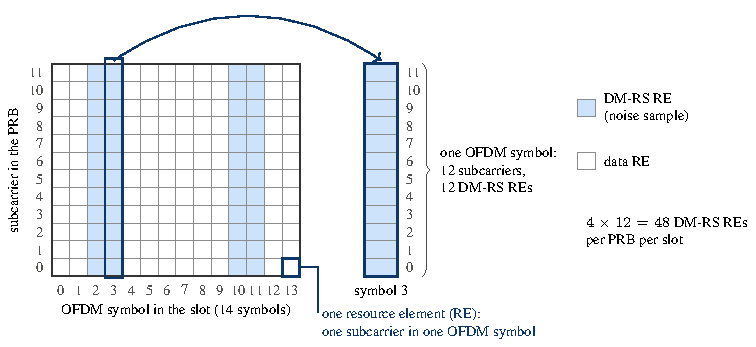
\includegraphics{Images/FLUXO/prb_dmrs.pdf}
\vspace{4pt}
\legend{Source: the author, with the DM-RS positions of \citesp{3gpp-ts38211}. \textcolor{red}{Double-symbol DM-RS}, mapping type~A, symbols 2, 3, 10 and 11.}
\end{figure}


A sample represents the noise covariance for a given data symbol only if both fall within the same interval of duration $T_c$. As a result, the number of available samples may vary from one data symbol to another. For any given symbol, the number of samples corresponds to the maximum count of DM-RS REs found within an interval of duration $T_c$ that encompasses that symbol. The number of samples available for all symbols in the slot is the smallest of these values. Figure~\ref{fig:dmrs-n} shows an example with the DM-RS located at symbols 2, 3, 10, and 11 of each slot. Under the TDLB100-400 condition, symbols 5 through 8 represent the worst-case scenario, with 24 samples. Therefore, the number of samples available for all symbols is 24. Table~\ref{tab:n-maximo} presents this value for each test condition.

\begin{table}[htbp]
\caption{Number of DM-RS REs per PRB available to every data symbol of the slot, in each test condition.}
\label{tab:n-maximo}
\vspace{4pt} % a classe zera o espaço entre a caption e a tabela
\centering
\footnotesize
\renewcommand{\arraystretch}{1.2}
\setlength{\aboverulesep}{0pt}
\setlength{\belowrulesep}{0pt}
\begin{tabular}{|c|c|c|c|c|}
\toprule
\multirow{2}{*}{\textbf{Test condition}} & \textbf{Frequency} & \multirow{2}{*}{{\boldmath $T_c$} \textbf{(ms)}} & \textbf{OFDM symbols} & \textbf{DM-RS REs} \\
 & \textbf{range} & & \textbf{in} {\boldmath $T_c$} & \textbf{available} \\
\midrule
TDLA30-5    & \multirow{2}{*}{FR1} & 25.0000 & 700 & 2400 \\
TDLA30-10   &                      & 12.5000 & 350 & 1200 \\
\cline{2-2}
TDLA30-75   & \multirow{2}{*}{FR2} & 1.6667  & 186 & 648 \\
TDLA30-300  &                      & 0.4167  & 46  & 168 \\
\cline{2-2}
TDLC300-100 & \multirow{4}{*}{FR1} & 1.2500  & 35  & 132 \\
TDLB100-400 &                      & 0.3125  & 8   & 24 \\
HST350      &                      & 0.0536  & \multirow{2}{*}{1} & \multirow{2}{*}{0} \\
HST500      &                      & 0.0375  &     &  \\
\bottomrule
\end{tabular}
\vspace{4pt}
\legend{Source: the author, from \citesp{3gpp-ts38104}; \citesp{3gpp-ts38211}; \citesp{tse-viswanath}. \textcolor{red}{Double-symbol DM-RS} in symbols 2, 3, 10 and 11, with every slot carrying PUSCH.}
\end{table}

The best range of a data symbol may include DM-RS that arrive after that symbol. In Figure ~\ref{fig:dmrs-n}(b), the best range of symbol 13 goes up to symbol 3 of the next slot. To use these samples, the receiver needs to store symbol 13 for 4 more symbols.
% Figura: de onde vem o N de uma condição de teste (2026-11-04).
%   (a) pior caso (símbolo 6) e (b) melhor caso (símbolo 13): as 8 posições de um
%       intervalo de T_c = 8 símbolos (TDLB100-400) que contêm o símbolo.
%   A antiga parte (a), o PRB em um slot, virou a Figura fig:prb-dmrs (fig-prb-dmrs.tex).
%   Contagens geradas em Python (DM-RS em {2,3,10,11}, slots contínuos, L = 8).
%   Cores repetidas de fig-prb-dmrs.tex, para a figura não depender da ordem.
\definecolor{dmrsfill}{HTML}{CDE2FB}
\definecolor{winblue}{HTML}{0D366B}
\definecolor{inksec}{HTML}{52514E}
\begin{figure}[htbp]
\caption{Intervals of duration $T_c$ that contain a data symbol, and their DM-RS REs per PRB, in the TDLB100-400 condition.}
\label{fig:dmrs-n}
\vspace{4pt} % a classe zera o espaço entre a caption e a figura
\centering
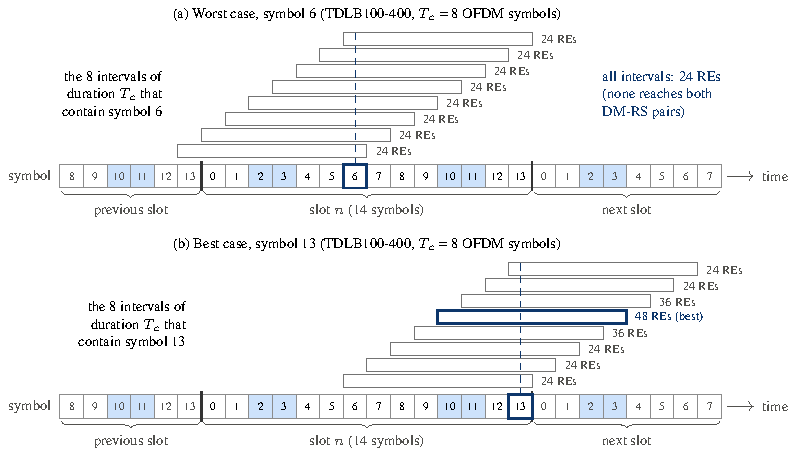
\includegraphics{Images/FLUXO/dmrs_n.pdf}
\vspace{4pt}
\legend{Source: the author, with the DM-RS positions of \citesp{3gpp-ts38211}. \textcolor{red}{Double-symbol DM-RS}, mapping type~A, symbols 2, 3, 10 and 11; continuous uplink. In (a) and (b), each bar is one position of an interval of duration $T_c$ that contains the marked symbol. Symbol 6 is the worst case of the slot, and symbol 13 is a best case.}
\end{figure}



\subsubsection{Condicionamento da estimativa}\label{subsubsec:condicionamento-R}
% ANTIGO:
% O posto de uma matriz é o número máximo de linhas ou colunas linearmente independentes que essa matriz possui.  Cada parcela $\mathbf{n}^i(\mathbf{n}^i)^H$ é uma matriz de posto unitário, uma vez que todas as suas colunas são múltiplas do mesmo vetor $\mathbf{n}^i$. Consequentemente, o posto da soma de (N) desses produtos é limitado por (N):
\textcolor{red}{O posto de uma matriz é o número máximo de linhas ou colunas linearmente independentes. Cada parcela $\mathbf{n}^i(\mathbf{n}^i)^H$ tem posto 1, porque todas as suas colunas são múltiplas de $\mathbf{n}^i$. Então, o posto da soma de $N$ parcelas é no máximo $N$:}

\[
\operatorname{rank}(\widehat{\mathbf R}_n) \leq \min(M,N)
\]

% ANTIGO:
% Assim, quando (N<M), a estimativa amostral da matriz completa $(M\times M)$ é necessariamente singular. Uma matriz singular não é inversível. Essa propriedade precisa ser considerada em operações que exigem a inversão da matriz de covariância.
%
% \cite{zhao2025jsac} adota a condição $N\gg K$, para obter uma estimativa suficientemente precisa. Em suas simulações, utiliza (N=192) amostras por realização do canal. Um trabalho anterior dos mesmos autores também apresenta 96 e 192 como valores típicos para essa quantidade de amostras (Zhao et al., 2021).
\textcolor{red}{Assim, quando $N<M$, $\widehat{\mathbf R}_n$ é singular e não tem inversa.}

\textcolor{red}{O artigo base adota $N\gg K$ para obter uma estimativa precisa e usa $N=192$ amostras por realização do canal \cite{zhao2025jsac}. Um trabalho anterior dos mesmos autores cita 96 e 192 como valores típicos \cite{zhao2021-globecom}.}

% SEPARAÇÃO (2026-11-04): explicação do Ledoit-Wolf trazida de METODOLOGIA/simulacao.tex.
\textcolor{red}{Uma forma de tornar a estimativa inversível é o encolhimento (\textit{shrinkage}) de Ledoit e Wolf. Ele troca $\hat{\mathbf R}_n$ por uma média ponderada entre $\hat{\mathbf R}_n$ e um múltiplo da identidade \cite{ledoit-wolf}:}
\begin{equation}
\hat{\mathbf R}_{\text{LW}}=(1-\textcolor{red}{\alpha})\,\hat{\mathbf R}_n+\textcolor{red}{\alpha}\,\mu\,\mathbf I_M,
\qquad
\mu=\frac{\operatorname{tr}(\hat{\mathbf R}_n)}{M}.
\label{eq:ledoit-wolf}
\end{equation}
\textcolor{red}{O peso $\alpha$, entre 0 e 1, é calculado a partir das próprias amostras, de forma a minimizar o erro quadrático esperado entre a estimativa e a covariância verdadeira \cite{ledoit-wolf}. Como $\hat{\mathbf R}_n$ não tem autovalores negativos, todo autovalor de $\hat{\mathbf R}_{\text{LW}}$ é pelo menos $\alpha\mu$. Quando $\alpha > 0$, a matriz resultante é inversível.}
% FONTE: Ledoit e Wolf (2004), alvo mu I com mu = tr/M e alpha estimado das amostras
%   (TODO: conferir número da equação/página). Simulador: m5_noise.shrink.
% NOSSO (conta): autovalores de (1-alpha)R + alpha mu I = (1-alpha) lambda_i + alpha mu >= alpha mu.
% FORA (sem fonte): a alternativa da carga diagonal com epsilon fixo.





